% GeoCrop - FYP poster (F26-155). 22.5in x 34.5in, portrait.
% Build: pdflatex poster.tex
\documentclass{article}
\usepackage{fix-cm}
\usepackage[paperwidth=22.5in,paperheight=34.5in,margin=0in]{geometry}
\usepackage[T1]{fontenc}
\usepackage[scaled=1]{helvet}
\renewcommand{\familydefault}{\sfdefault}
\usepackage{graphicx,xcolor,array}
\usepackage{tikz}
\usetikzlibrary{arrows.meta,positioning,shapes.geometric,calc,fit,backgrounds}
\usepackage{pgfplots}
\pgfplotsset{compat=1.18}
\pgfkeys{/pgf/number format/assume math mode=true}
\pagestyle{empty}
\setlength{\parindent}{0pt}

% ---------------------------------------------------------------- palette
\definecolor{forest}{HTML}{1F5130}
\definecolor{leaf}{HTML}{2E7D32}
\definecolor{lime}{HTML}{8BC34A}
\definecolor{wheat}{HTML}{F2A900}
\definecolor{soil}{HTML}{8D5A3B}
\definecolor{sky}{HTML}{1E6FA8}
\definecolor{paper}{HTML}{F4F7F1}
\definecolor{ink}{HTML}{1B1F1C}
\definecolor{muted}{HTML}{4F5B52}
\definecolor{alert}{HTML}{B3261E}

% ---------------------------------------------------------------- type scale (readable from 1 m)
\newcommand{\bodyfont}{\fontsize{27}{35}\selectfont}
\newcommand{\smallfont}{\fontsize{22}{28}\selectfont}
\newcommand{\tinyfont}{\fontsize{19}{24}\selectfont}
\newcommand{\headfont}{\fontsize{40}{46}\selectfont\bfseries}
\newcommand{\bignum}{\fontsize{64}{66}\selectfont\bfseries}

% ---------------------------------------------------------------- helpers
% \panel{x1}{ytop}{x2}{ybottom}{title}   (y measured from the top of the page, inches)
\newcommand{\panel}[5]{%
  \fill[white, rounded corners=14pt, drop shadow/.style={}] (#1,{34.5-(#2)}) rectangle (#3,{34.5-(#4)});
  \draw[forest!35, line width=2pt, rounded corners=14pt] (#1,{34.5-(#2)}) rectangle (#3,{34.5-(#4)});
  \fill[forest, rounded corners=14pt] (#1,{34.5-(#2)}) rectangle (#3,{34.5-(#2)-0.95});
  \fill[forest] (#1,{34.5-(#2)-0.5}) rectangle (#3,{34.5-(#2)-0.95});
  \fill[wheat] (#1+0.35,{34.5-(#2)-0.3}) rectangle ++(0.14,-0.38);
  \node[anchor=west, text=white, inner sep=0] at (#1+0.7,{34.5-(#2)-0.48}) {\headfont #5};
}
\newcommand{\at}[2]{(#1,{34.5-(#2)})}
\tikzset{
  flow/.style={draw=forest, line width=2pt, rounded corners=10pt, fill=paper, align=center,
               text width=#1, inner sep=10pt, font=\smallfont},
  flow/.default=5.8in,
  svc/.style={draw=forest, line width=2pt, rounded corners=10pt, fill=lime!18, align=center,
              text width=#1, minimum height=1.25in, inner sep=8pt, font=\smallfont},
  svc/.default=3.4in,
  db/.style={draw=forest, line width=2pt, cylinder, shape border rotate=90, aspect=0.2,
             fill=sky!12, align=center, minimum width=3.2in, minimum height=1.35in, font=\smallfont},
  ar/.style={-{Latex[length=16pt,width=13pt]}, line width=3pt, forest},
  dar/.style={-{Latex[length=16pt,width=13pt]}, line width=3pt, dashed, forest!70},
  chip/.style={draw=none, rounded corners=9pt, fill=#1, text=white, font=\smallfont\bfseries,
               inner xsep=12pt, inner ysep=8pt},
  chip/.default=leaf,
  lbl/.style={font=\tinyfont, fill=white, inner sep=3pt, text=muted},
}

% ---------------------------------------------------------------- project logo (designed for GeoCrop)
\newcommand{\geocroplogo}{%
  \fill[white] (0,0) circle (1.08);
  \begin{scope}
    \clip (0,0) circle (1);
    \fill[forest] (-1,-1) rectangle (1,1);
    % field parcels seen from orbit
    \fill[wheat]  (-1.2,-1.2) -- (0.05,-1.2) -- (-0.35,-0.05) -- (-1.2,0.25) -- cycle;
    \fill[lime]   (0.15,-1.2) -- (1.2,-1.2) -- (1.2,-0.2) -- (-0.25,-0.05) -- cycle;
    \fill[soil]   (-1.2,0.35) -- (-0.3,0.05) -- (-0.05,0.55) -- (-1.2,0.95) -- cycle;
    \fill[leaf]   (-0.15,0.05) -- (1.2,-0.1) -- (1.2,0.75) -- (0.05,0.6) -- cycle;
    \draw[white, line width=2.5pt] (-1.2,0.3) -- (-0.32,0.0) -- (0.1,-1.2);
    \draw[white, line width=2.5pt] (-0.32,0.0) -- (1.2,-0.15);
    \draw[white, line width=2.5pt] (-0.2,0.05) -- (0.0,0.6) -- (-1.2,1.0);
    % leaf / map pin
    \fill[white] (0.32,0.05) .. controls (0.95,0.25) and (0.9,0.85) .. (0.32,1.05)
                 .. controls (-0.25,0.85) and (-0.3,0.25) .. (0.32,0.05) -- cycle;
    \draw[leaf, line width=2.5pt] (0.32,0.12) .. controls (0.30,0.5) .. (0.36,0.98);
  \end{scope}
  % satellite orbit
  \draw[wheat, line width=5pt] (0,0) ++(185:1.22) arc (185:305:1.22);
  \begin{scope}[shift={(305:1.22)}, rotate=35]
    \fill[white, draw=forest, line width=1.5pt] (-0.09,-0.07) rectangle (0.09,0.07);
    \fill[sky]  (-0.32,-0.05) rectangle (-0.12,0.05);
    \fill[sky]  (0.12,-0.05) rectangle (0.32,0.05);
  \end{scope}
}

\begin{document}
\begin{tikzpicture}[x=1in, y=1in, inner sep=0]
% ---------------------------------------------------------------- canvas
\fill[paper] (0,0) rectangle (22.5,34.5);

% ================================================================= HEADER
\fill[forest] \at{0}{0} rectangle \at{22.5}{4.5};
\fill[wheat]  \at{0}{4.5} rectangle \at{22.5}{4.66};
\begin{scope}[shift={(2.7,{34.5-2.2})}, x=1cm, y=1cm, scale=4.0]\geocroplogo\end{scope}
\node[anchor=west, text=white, inner sep=0] at \at{4.95}{1.4}
  {\fontsize{118}{118}\selectfont\bfseries Geo\textcolor{wheat}{Crop}};
\node[anchor=west, text=white, inner sep=0] at \at{5.02}{2.85}
  {\fontsize{37}{44}\selectfont Automated Crop Monitoring and Forecasting Toolkit};
\node[anchor=west, text=white!82!forest, inner sep=0] at \at{5.04}{3.72}
  {\fontsize{25}{30}\selectfont Final Year Project \;|\; F26-155 \;|\; Department of Computer Science};
\fill[white, rounded corners=16pt] \at{18.2}{0.45} rectangle \at{21.85}{4.05};
\node at \at{20.03}{1.85} {
\includegraphics[width=2.0in]{figures/fast_logo.png}};
\node[align=center, text=forest, font=\fontsize{21}{24}\selectfont\bfseries] at \at{20.03}{3.5}
  {FAST NUCES\\[-2pt]Islamabad Campus};

% ================================================================= OBJECTIVE
\fill[white, rounded corners=14pt] \at{0.7}{4.95} rectangle \at{21.8}{6.75};
\draw[wheat, line width=3pt, rounded corners=14pt] \at{0.7}{4.95} rectangle \at{21.8}{6.75};
\fill[wheat, rounded corners=14pt] \at{0.7}{4.95} rectangle \at{4.6}{6.75};
\fill[wheat] \at{4.0}{4.95} rectangle \at{4.6}{6.75};
\node[text=forest, align=center, font=\fontsize{40}{44}\selectfont\bfseries] at \at{2.65}{5.85} {Objective};
\node[anchor=west, text width=16.6in, text=ink, font=\fontsize{31}{40}\selectfont] at \at{4.95}{5.85}
  {Turn raw \textbf{Sentinel-2 satellite imagery} into \textbf{cropland, crop-type, field and yield
   layers} on a \textbf{lightweight web map} that stays fast as images and models grow.};

% ================================================================= ROW 1: PROBLEM | ARCHITECTURE
\panel{0.7}{7.15}{8.45}{15.55}{Problem Overview}
\node[anchor=north west, text width=7.0in, font=\bodyfont, text=ink] at \at{1.1}{8.35}
  {Crop surveys still depend on field visits and hand-drawn GIS maps.};
\node[font=\smallfont\bfseries, text=alert, anchor=west] at \at{1.1}{9.75} {TODAY};
\node[flow=6.6in, fill=alert!8, draw=alert, anchor=north] (t1) at \at{4.57}{10.05}
  {Field visits $\rightarrow$ manual crop identification $\rightarrow$ hand-drawn boundaries};
\node[font=\smallfont, text=alert, anchor=north, text width=6.6in, align=center] at \at{4.57}{11.25}
  {slow \;$\cdot$\; costly \;$\cdot$\; hard to repeat every season};
\node[font=\smallfont\bfseries, text=leaf, anchor=west] at \at{1.1}{12.05} {WITH GEOCROP};
\node[flow=6.6in, fill=lime!18, anchor=north] (g1) at \at{4.57}{12.3} {Upload a Sentinel-2 image};
\node[flow=6.6in, fill=lime!18, anchor=north] (g2) at \at{4.57}{13.25} {Models: cropland $\rightarrow$ crop type $\rightarrow$ fields $\rightarrow$ yield};
\node[flow=6.6in, fill=wheat!30, draw=wheat!70!black, anchor=north] (g3) at \at{4.57}{14.4} {\textbf{Map layers + statistics in about 1 minute}};
\draw[ar] (g1) -- (g2); \draw[ar] (g2) -- (g3);

\panel{8.85}{7.15}{21.8}{15.55}{System Architecture}
\node[anchor=north west, font=\bodyfont, text=ink, text width=12.2in] at \at{9.25}{8.35}
  {Design principle: \textbf{\textcolor{leaf}{send only what is visible}}. Results are stored once
   as rasters; the browser loads only the small map tiles in view.};
\node[svc=11.6in, minimum height=0.9in, fill=lime!30] (web) at \at{15.32}{10.2}
  {\textbf{Web GIS client}: React + MapLibre GL (WebGL)};
\node[svc=11.6in, minimum height=0.85in, fill=wheat!28] (nginx) at \at{15.32}{11.5}
  {\textbf{Nginx}: serves the app, routes requests, \textbf{caches tiles}};
\node[svc] (api)    at \at{11.38}{13.0} {\textbf{FastAPI}\\catalogue, stats, uploads};
\node[svc] (tiles)  at \at{15.32}{13.0} {\textbf{TiTiler}\\COG $\rightarrow$ map tiles};
\node[svc] (worker) at \at{19.26}{13.0} {\textbf{Celery workers}\\plug-in model registry};
\node[db] (pg)    at \at{11.38}{14.65} {PostGIS};
\node[db] (minio) at \at{15.32}{14.65} {MinIO (S3)\\[-4pt]{\tinyfont COG, PMTiles}};
\node[db] (redis) at \at{19.26}{14.65} {Redis\\[-4pt]{\tinyfont job queue}};
\draw[ar] (web) -- (nginx);
\draw[ar] (nginx.south -| api.north) -- (api.north);
\draw[ar] (nginx.south -| tiles.north) -- (tiles.north);
\draw[ar] (api) -- (pg);
\draw[ar] (tiles) -- (minio);
\draw[ar] (worker) -- (redis);
\draw[ar] (worker.south west) -- (minio.north east);
\draw[dar] (api.east) -- (tiles.west);
\draw[dar] (tiles.east) -- (worker.west);

% ================================================================= ROW 2: RESULTS
\panel{0.7}{15.95}{11.05}{22.35}{Rendering Performance}
\node[anchor=north west, text width=9.6in, font=\smallfont, text=ink] at \at{1.1}{17.1}
  {Map data downloaded for \textbf{one screen} of AOI 1 (log scale). The prototype sent one file with \textbf{101,435 polygons}.};
\begin{scope}[shift={(2.6,{34.5-19.95})}]
\begin{axis}[xbar, xmode=log, width=8.0in, height=2.25in, scale only axis=false, bar width=0.42in,
  symbolic y coords={Platform,Prototype}, ytick={Platform,Prototype}, xmin=100, xmax=600000, xtick={100,1000,10000,100000}, xticklabels={100 KB,1 MB,10 MB,100 MB},
  y tick label style={font=\smallfont\bfseries}, x tick label style={font=\tinyfont},
  axis x line*=bottom, axis y line*=left, enlarge y limits=0.5, line width=1.5pt]
\addplot[fill=leaf, draw=none, bar shift=0pt] coordinates {(337,Platform)};
\addplot[fill=alert!80, draw=none, bar shift=0pt] coordinates {(43300,Prototype)};
\node[anchor=west, font=\smallfont\bfseries] at (axis cs:337,Platform) {\;337 KB};
\node[anchor=west, font=\smallfont\bfseries] at (axis cs:43300,Prototype) {\;43.3 MB};
\end{axis}
\end{scope}
\foreach \x/\n/\t in {2.4/130$\times$/less data per screen, 5.88/47 ms/new tile (1 ms cached), 9.35/57 s/upload to map}{
  \node[text=forest, font=\bignum] at \at{\x}{21.15} {\n};
  \node[text=muted, font=\tinyfont] at \at{\x}{21.85} {\t};
}

\panel{11.45}{15.95}{21.8}{22.35}{Crop-Type Model Evaluation}
\node[anchor=north west, text width=9.6in, font=\smallfont, text=ink] at \at{11.85}{17.1}
  {\textbf{11 models} compared on spatially separated test blocks (USDA CDL labels).
   \textbf{LightGBM selected}: about \textbf{2 MB}, CPU only; Presto foundation model 660$\times$ slower.};
\begin{scope}[shift={(13.1,{34.5-21.3})}]
\begin{axis}[ybar, width=8.4in, height=2.9in, bar width=0.8in, ymin=0, ymax=112,
  symbolic x coords={A,B,C,D}, xtick=data,
  xticklabels={{1 date, AOI 1},{12 months, AOI 1},{LightGBM, AOI 1},{LightGBM, AOI 2}},
  x tick label style={font=\tinyfont, text width=1.8in, align=center},
  y tick label style={font=\tinyfont}, ylabel={Accuracy (\%)}, ylabel style={font=\tinyfont},
  ytick={0,25,50,75,100}, yticklabels={0,25,50,75,100},
  axis x line*=bottom, axis y line*=left, line width=1.5pt,
  nodes near coords={\pgfmathprintnumber{\pgfplotspointmeta}\%}, nodes near coords style={font=\smallfont\bfseries},
  enlarge x limits=0.17]
\addplot[fill=leaf, draw=none] coordinates {(A,26.7) (B,75.2) (C,76.1) (D,92.2)};
\end{axis}
\end{scope}

% ================================================================= ROW 3: PLAN
\panel{0.7}{22.75}{21.8}{27.65}{Iterative Project Plan}
\node[anchor=north west, font=\smallfont, text=muted] at \at{1.1}{23.9}
  {Every iteration delivers a working, demonstrable outcome. Two parallel tracks: platform architecture and model research.};
\foreach \i/\x/\c/\when/\stat/\what/\out in {
  1/1.1/leaf/{Sep--Oct 2026 (FYP-I)}/DONE/{Base architecture + performance benchmark; 11 crop-type models evaluated}/{Working platform v1},
  2/6.3/wheat!85!black/{Oct--Dec 2026 (FYP-I)}/IN PROGRESS/{LightGBM in platform; cross-area test; multi-image upload; usability study}/{Platform v2},
  3/11.5/sky/{Feb--Mar 2027 (FYP-II)}/PLANNED/{Field-boundary model; yield model (USDA NASS); more areas}/{Boundary + yield layers},
  4/16.7/muted/{Apr--May 2027 (FYP-II)}/PLANNED/{End-to-end evaluation; hardening; cloud deployment}/{Deployed release}}{
  \fill[\c, rounded corners=10pt] \at{\x}{24.5} rectangle \at{\x+4.75}{25.35};
  \node[text=white, font=\smallfont\bfseries, anchor=west] at \at{\x+0.25}{24.925} {Iteration \i};
  \node[text=white, font=\tinyfont\bfseries, anchor=east] at \at{\x+4.55}{24.925} {\stat};
  \node[anchor=north west, text width=4.5in, font=\tinyfont\bfseries, text=muted] at \at{\x+0.12}{25.5} {\when};
  \node[anchor=north west, text width=4.5in, font=\tinyfont, text=ink] at \at{\x+0.12}{25.95} {\what};
  \node[anchor=north west, text width=4.5in, font=\smallfont\bfseries, text=\c] at \at{\x+0.12}{26.95} {$\Rightarrow$ \out};
}
\foreach \x in {5.9,11.1,16.3}{ \draw[ar, line width=4pt] \at{\x}{24.925} -- \at{\x+0.36}{24.925}; }

% ================================================================= ROW 4: SCREENS | TOOLS
\panel{0.7}{28.05}{10.45}{32.0}{Live Map and Dashboard}
\node[anchor=north west, draw=forest!40, line width=1pt, inner sep=0] at \at{1.0}{29.25} {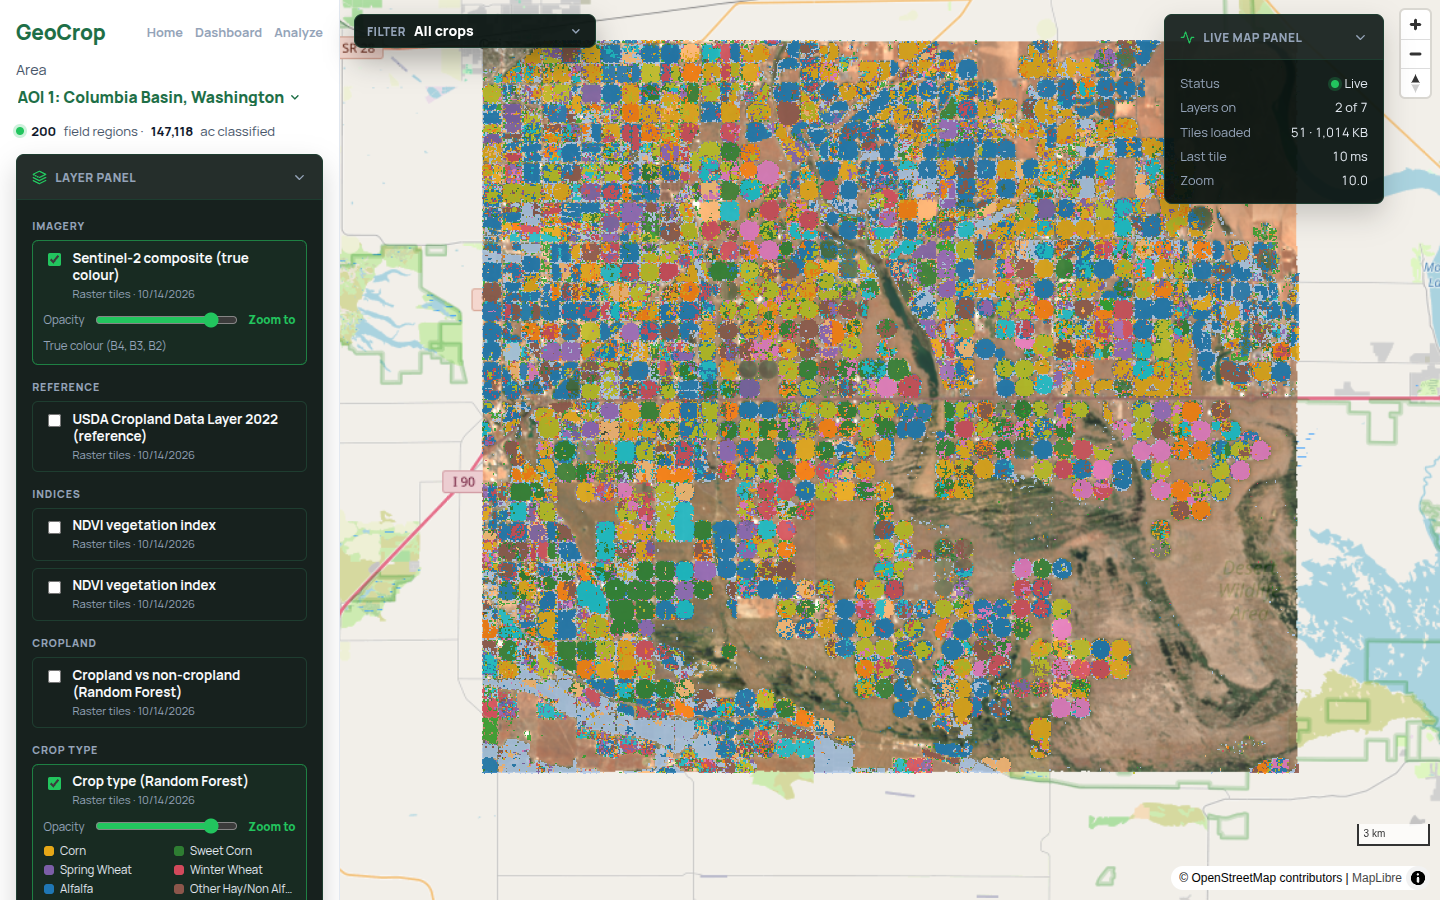
\includegraphics[width=4.45in]{figures/shot_map.png}};
\node[anchor=north west, draw=forest!40, line width=1pt, inner sep=0] at \at{5.7}{29.25} {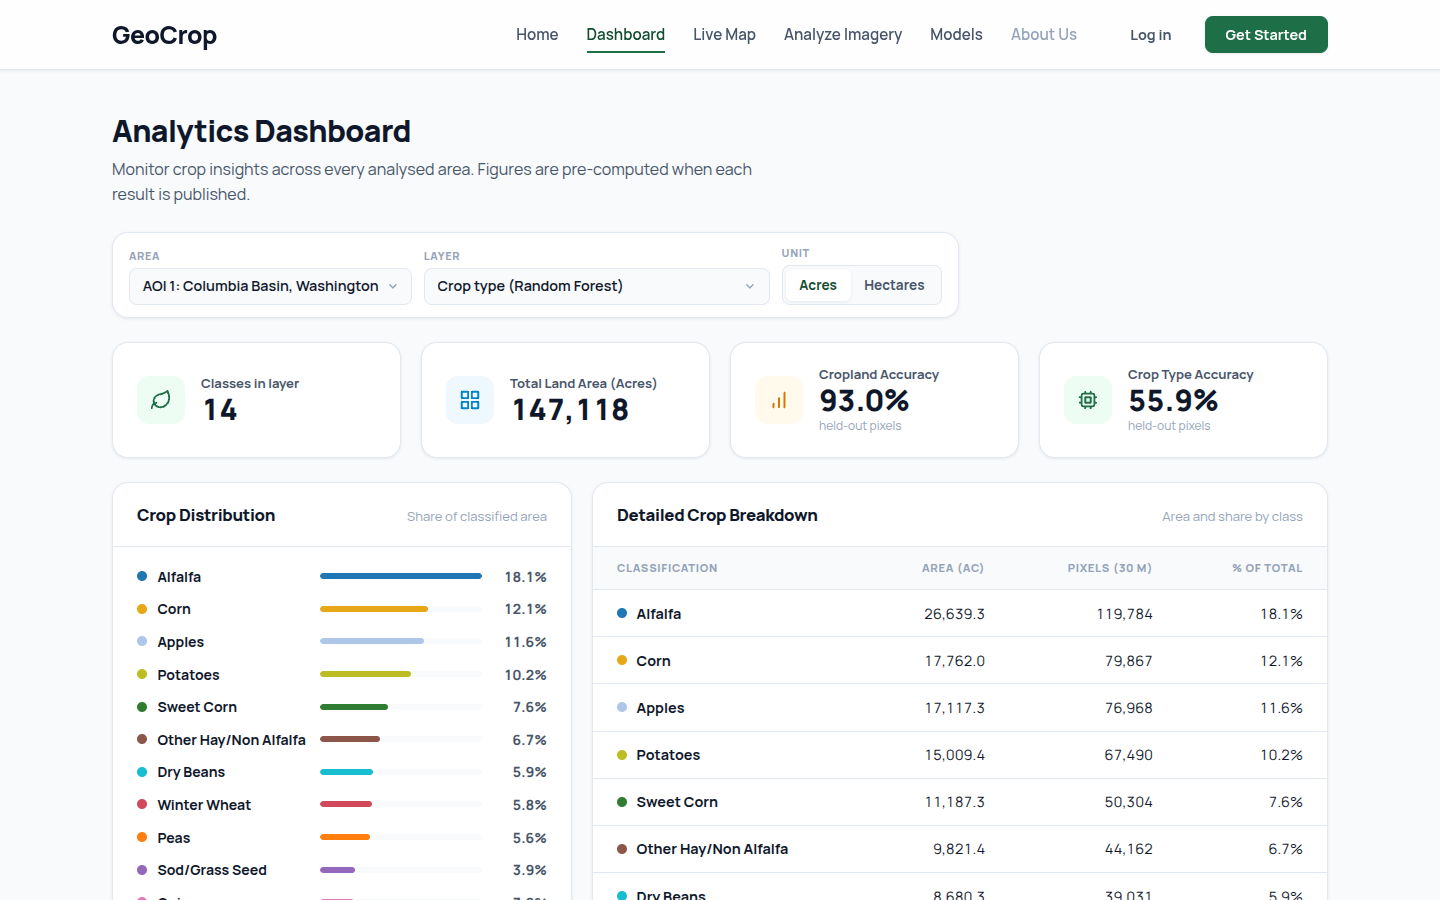
\includegraphics[width=4.45in]{figures/shot_dashboard.png}};

\panel{10.85}{28.05}{21.8}{32.0}{Tools \& Technologies}
\node[anchor=north west, text width=10.4in, font=\smallfont, align=left] at \at{11.2}{29.3} {%
  \tikz[baseline]\node[chip=leaf]{React}; \tikz[baseline]\node[chip=leaf]{MapLibre GL};
  \tikz[baseline]\node[chip=leaf]{FastAPI}; \tikz[baseline]\node[chip=leaf]{Celery + Redis};
  \tikz[baseline]\node[chip=leaf]{Nginx};\\[16pt]
  \tikz[baseline]\node[chip=sky]{PostgreSQL + PostGIS}; \tikz[baseline]\node[chip=sky]{TiTiler (COG)};
  \tikz[baseline]\node[chip=sky]{PMTiles}; \tikz[baseline]\node[chip=sky]{MinIO (S3)};\\[16pt]
  \tikz[baseline]\node[chip=soil]{LightGBM}; \tikz[baseline]\node[chip=soil]{scikit-learn};
  \tikz[baseline]\node[chip=soil]{Sentinel-2 + USDA CDL}; \tikz[baseline]\node[chip=forest]{Docker};};

% ================================================================= FOOTER: TEAM
\fill[wheat]  \at{0}{32.3} rectangle \at{22.5}{32.46};
\fill[forest] \at{0}{32.46} rectangle \at{22.5}{34.5};
\node[anchor=west, text=wheat, font=\headfont] at \at{0.75}{33.0} {Team};
\node[anchor=west, text=white, font=\fontsize{26}{30}\selectfont] at \at{3.1}{33.0}
  {\textbf{Huzaifa Bin Khalid} \;(22I-2332) \quad \textbf{Taha Bashir Awan} \;(23I-0824) \quad \textbf{Saneed Ullah} \;(23I-2568)};
\node[anchor=west, text=white, font=\fontsize{24}{28}\selectfont] at \at{0.75}{33.85}
  {\textcolor{wheat}{\textbf{Supervisor:}} Mr. Muhammad Aadil Ur Rehman \qquad
   \textcolor{wheat}{\textbf{Co-Supervisor:}} Mr. Obaid Ur Rehman (Institute of Space Technology)};
\fill[white, rounded corners=8pt] \at{20.25}{32.62} rectangle \at{21.95}{34.32};
\node at \at{21.1}{33.47} {
\includegraphics[width=1.55in]{figures/qr_repo.png}};
\node[anchor=east, text=white!80!forest, font=\tinyfont] at \at{20.1}{34.25} {Source code};
\end{tikzpicture}
\end{document}
